\documentclass[11pt]{article}

\usepackage{multirow}
\usepackage{subfig}
\usepackage{xcolor}
\usepackage{listings}
\usepackage{graphicx}
\usepackage{amsmath}
\usepackage{hyperref}

\title{\textbf{Major Project Documentation}}
\author{Joe Withers}
\date{June 2018}

\lstset{ breaklines=true }

\begin{document}

\maketitle

\tableofcontents
\newpage

\section{Introduction}

This document serves to detail the work I was responsible for during the Final Major Project assignment, in which I helped create an animated short film as part of a four person team. My responsibilities during this project were mainly the technical aspects within production, such as pipeline development and rendering. In addition to this I was able to contribute to more artistic disciplines including character rigging, groom, and compositing.

\section{Pipeline Management}

As an aspiring software developer, I initially became interested in working on project as it gave me to design, develop, and implement a production pipeline for quite a complex project. From the beginning of the project I was eager to develop tools which would allow the production to be as efficient as possible, given that the scope of the project would require wrangling of large amounts of data across a large number of assets.

\subsection{Requirements}

\begin{itemize}

\item Reliably store all of the project data in such a way that is accessible to all team members.

\item Provide artists with a tool that manages assets, allowing them to update, reference,

\item Provide an automated method for caching the entire scene, with the aim of 'packaging' the project to make it suitable for rendering on different machines.

\end{itemize}

\subsection{Limitations}

Prior to developing the pipeline and associated tools, it was important to address the limitations imposed by the environment in which we would be working. The most important of these were:

\begin{itemize}

\item Lack of unified storage amongst users. Due to the way the university network is set up, it isn't possible to have a single network location for our shared data storage, without sacrificing one members allocated user storage.

\item Lack of storage per user. The approximate storage limit per user is 50gb, which would quickly be hit in a complex production environment. It is therefore imperative that we are conscious of the data that we keep hold of.

\item Lack of storage space on the render farm. The approximate storage limit on the render farm is 30gb, meaning that all of the data required to render a scene or shot must fit well within this limit, as rendered frames are written to the same location.

\end{itemize}

\subsection{Storage}

For file storage we chose to use Resilio Sync, a peer-to-peer file synchronisation service
to store all of our working files. This ensured that each team member has their own local copy of the entire working directory, which is beneficial when creating backups. We chose Resilio Sync primarily because it is a free service that is compatible with the university computer network, however it does present us with some problems.

Due to being it peer-to-peer service, we often found that directories would fail to synchronise properly if not synchronised frequently with the other peers. This would not be a problem in a cloud hosted service as the directory state of the working directory would be reliably centralised, reducing the possibility of files becoming desynchronised, however these services are typically expensive and it was difficult to predict our exact storage requirements.

We also noticed a strange problem with Resilio Sync, in which the contents of files would be reduced to 0 bytes. Fortunately the data is usually not lost as it is sent to the 'Archive', which functions as a temporary recycle bin, though restoring these files manually each time it happened proved to become quite tedious. I decided to write a simple bash script to check through the working directory to identify any files with a size of 0 bytes, and to check if a matching file was present in the Archive. However, this wasn't particularly effective as often they would be missing from both the main working directory and the Archive, meaning I would have to search through backups to find the file to restore, which at times felt a bit like baby-sitting.

\subsection{Asset Pipeline}

When establishing the asset pipeline it was important to separate pipeline steps not just by the type of work being done, but also by which of the team members is assigned to each discipline. Figure~\ref{figure:pipelineFlow} describes the flow of the data between pipeline steps and the corresponding team member(s) that they are assigned to.

\begin{figure}[htbp]\centering
	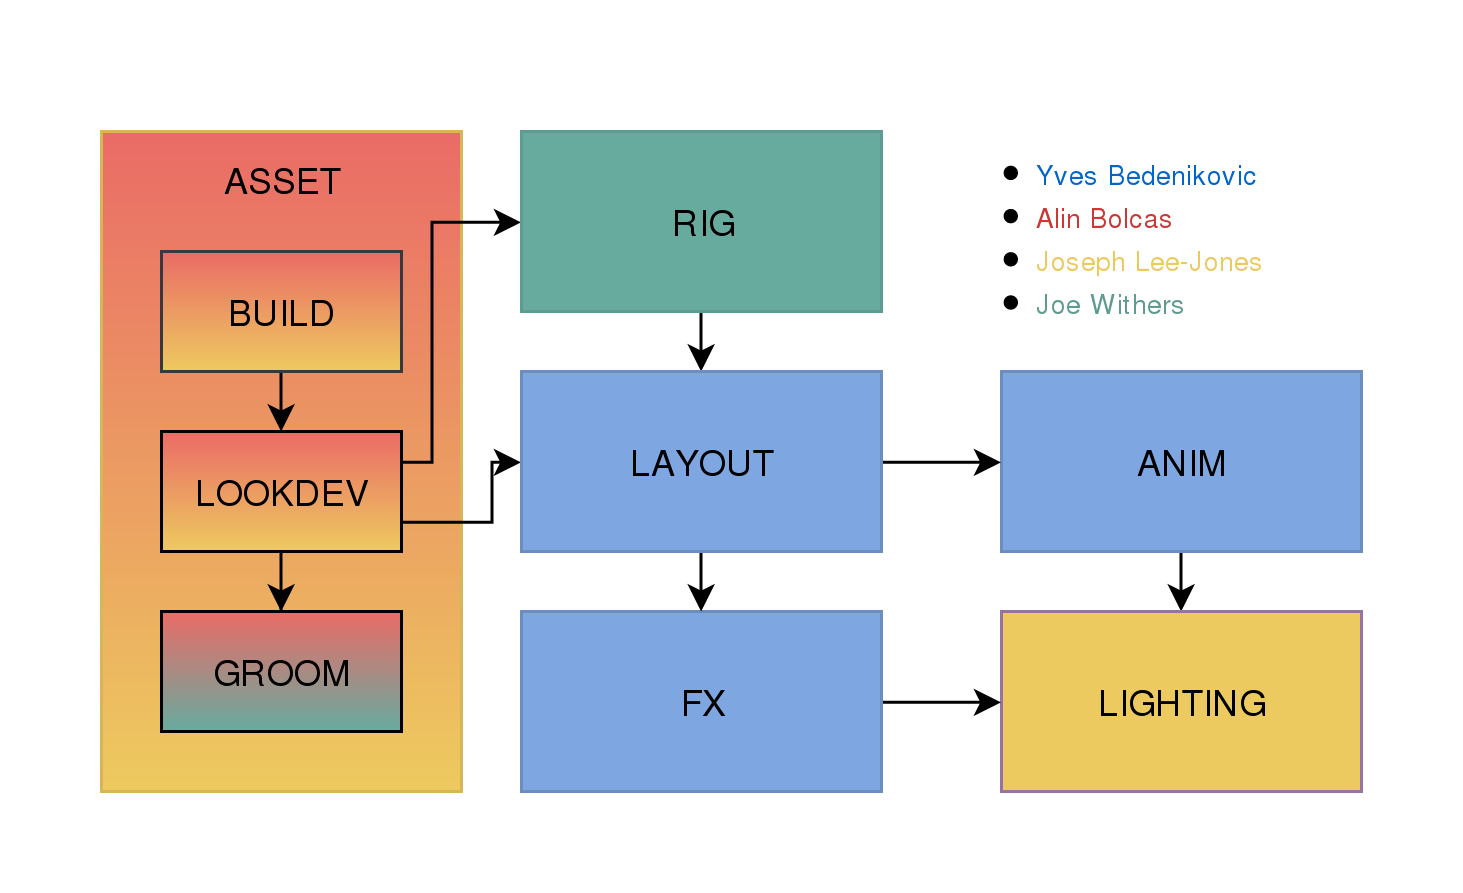
\includegraphics[width=1.0\linewidth]{images/pipeline.png}
	\caption{\label{figure:pipelineFlow} A Flowchart describing the asset pipeline, colours indicating the responsibilities of each group member.}
\end{figure}

\subsection{Asset Management} \label{assman}

With the Asset Pipeline established, I decided to design and develop an asset management system as it was clear that we would be working with a large number of assets. The asset management system would need to provide the following:

\begin{itemize}

\item Provide artists with a simple method for releasing new versions of assets.

\item Provide artists with a simple method for gathering assets, so that they can be referenced into a scene.

\item Manage versioning of assets, accompanied by information regarding each versions release date, author, and  description.

\item Automatically update references to assets whenever an asset or one of it's dependencies has been updated.

\end{itemize}

With this in mind I developed a system that made extensive use of symbolic links (Symlinks). Symlinks create a file which acts like a reference to another file. By creating a master symlink for each asset, updating the version of an asset is as simple as changing the target file. Files such as Maya scene files which contain references to existing file paths can have these paths substituted for symlinks, allowing me to change the version of any file in the asset pipeline non-destructively, with changes being propagated automatically. An example of data flow for multiple assets consisting of symlinks can be seen in Figure~\ref{figure:assetPipeline}.

\begin{figure}[htbp]\centering
	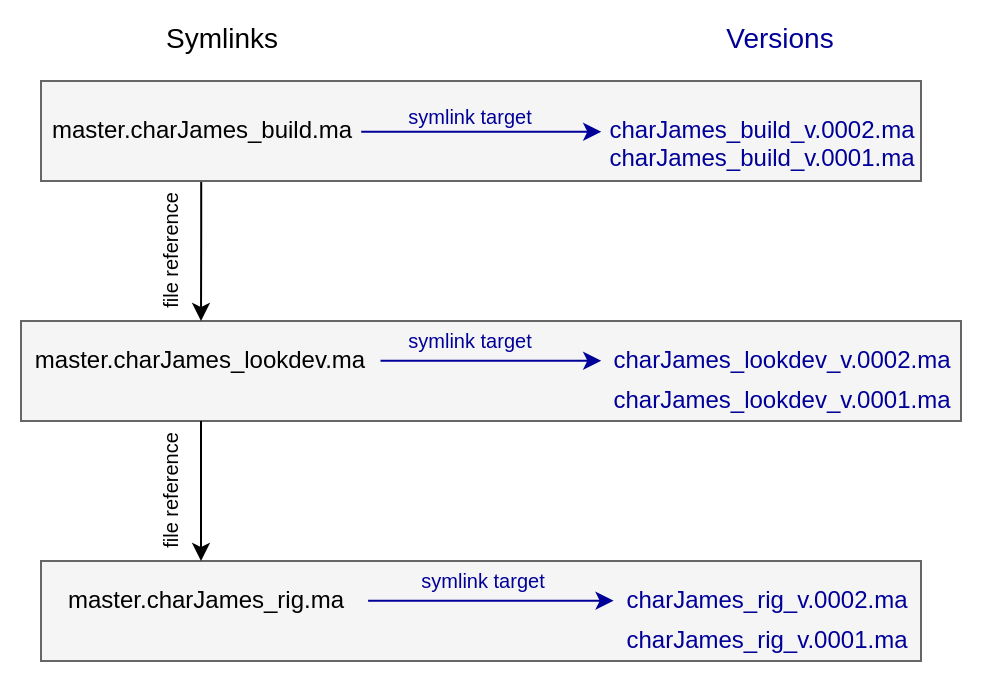
\includegraphics[width=1.0\linewidth]{images/asset_pipeline.png}
	\caption{\label{figure:assetPipeline} A Flowchart describing the data flow between pipeline steps for the 'charJames' asset. Note how the file versions for each pipeline step can be easily changed by re-targeting the symlink.}
\end{figure}

With this in place the next step was to develop a way of storing meta-data for each asset, so that a list of the released versions could be stored alongside important information about them, and that the current asset version could be easily identified. To implement this I created a simple Python dictionary that could be written to a file using the \texttt{cpickle} Python library~\cite{cpickle}; An example of the data stored within the asset file can be seen in Figure~\ref{figure:exampleAsset}.

\begin{figure}[htbp]\centering
	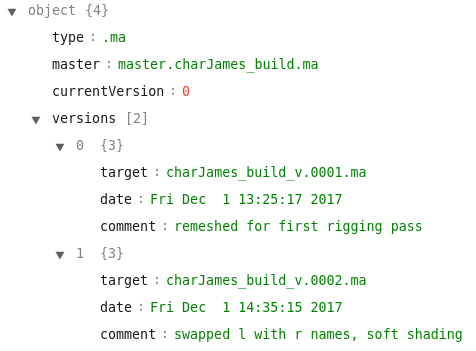
\includegraphics[width=0.8\linewidth]{images/assetExample.png}
	\caption{\label{figure:exampleAsset} An excerpt from the file \texttt{charJames\_build.asset}, showing how the data is structured.}
\end{figure}

The asset file contains the associated file type for the asset, the file name for the asset's symbolic link, and an index for where the current asset version is stored in the \texttt{versions} array. The \texttt{versions} array consists of Python dictionaries containing the target file name, the date of release, and a comment for each version in the array.

After testing this approach on a selection of non-production assets, I decided that this method of storing assets was fit for purpose, and decided to proceed by implementing a graphical asset manager that the other team members could use to author their own assets. For this I made use of Qt Designer to generate the user interface, primarily because I have experience using it to develop tools, but also because Maya 2017 supports Qt widgets with the inclusion of the PySide Python bindings. After multiple iterations per the requests of other team members, the GUI design shown in Figure~\ref{figure:assetManagerGui} was used for both the standalone version of the asset manager, and the Maya version which extends upon the functionality of the standalone version.

\begin{figure}[htbp]
\centering
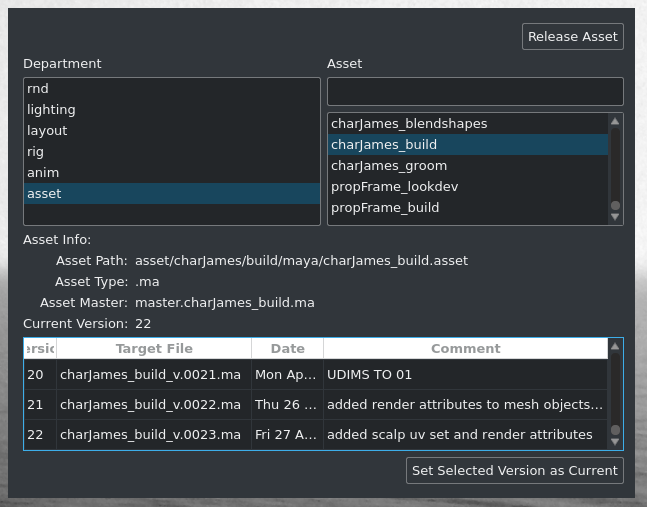
\includegraphics[width=0.8\linewidth]{images/amStandalone.png}
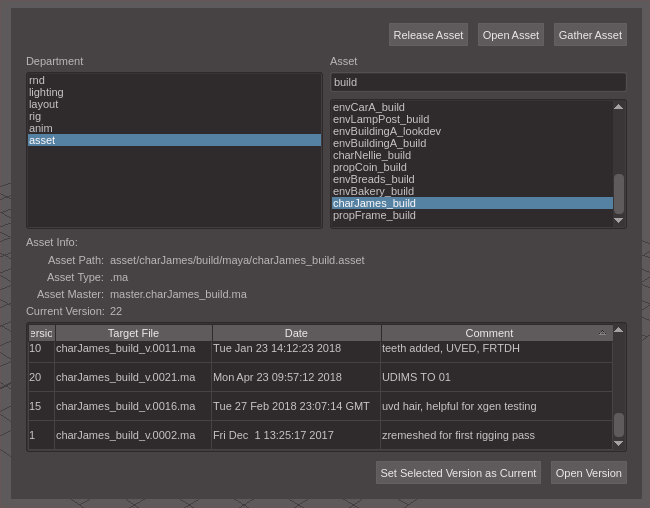
\includegraphics[width=0.8\linewidth]{images/amGuiMaya.png}
\caption{\label{figure:assetManagerGui} Comparison between the standalone version of the asset manager (Top), and the version of the asset manager designed for use within Autodesk Maya (Bottom). Note that the Maya version provides functionality for opening or 'gathering' assets directly into the current Maya session.}
\end{figure}

\subsection{Miscellaneous Tools}

During this project I was tasked with the development of a number of different tools and scripts per the requests of other team members. As a result I decided to implement a custom Maya shelf which all of the team members could install add to their Maya configuration. The shelf as seen in Figure~\ref{figure:shelf} provide the following functionality (In order from left to right):

\begin{itemize}

\item Access the Asset Manager, as described in section~\ref{assman}.

\item Release or cache a lighting scene, as described in section~\ref{rlslgt}.

\item Reference in an asset checker scene, used for test rendering assets under a variety of different HDRIs.

\item Dereference the asset checker scene.

\item Create a default set of groups in the outliner, as described by Yves Bedenikovic.

\item Set the environment variable used to store our project path as a RenderMan variable of the same value.

\item Change all texture paths in the scene to be absolute paths.

\item Change all texture paths in the scene to be paths relative to the environment variable used to store our project directory.

\item Fix any broken texture paths which have become broken as a result of team members using texture paths which are not relative to the project directory.

\item Print all texture paths into the script editor.

\item Generate viewport previews for all textures using UDIMS.

\item Automatically configure a new RenderMan PxrSurface shader, given a folder containing textures generated by Substance Painter or Substance Designer, as seen in Figure~\ref{figure:miscScripts}.

\item Load a 'character picker', which selects all of the facial or body controls on any of the rigs present in the scene, as seen in Figure~\ref{figure:miscScripts}.

\end{itemize}

\begin{figure}[htbp]
\centering

\includegraphics[width=1.0\linewidth]{images/shelf.png}
\caption{\label{figure:shelf} The custom Maya shelf created to provide all team members with easy access to the production tools and scripts.}
\end{figure}

\begin{figure}[htbp]
\centering
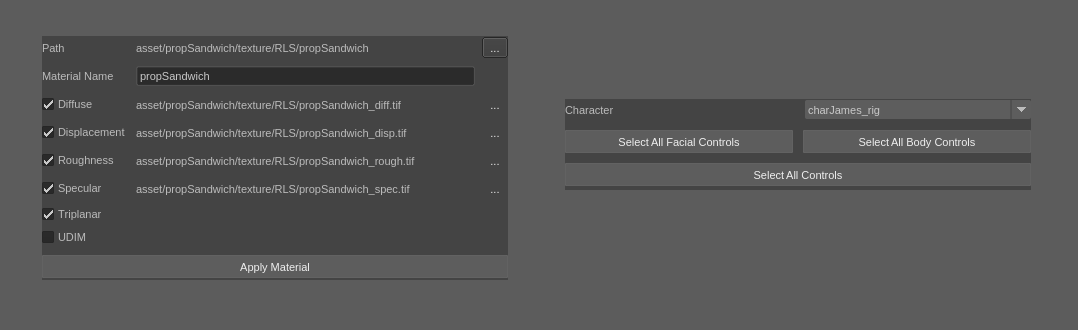
\includegraphics[width=1.0\linewidth]{images/miscScripts.png}
\caption{\label{figure:miscScripts} The tool I developed automatically configure a shader, given a folder containing textures generated by Substance Painter or Substance Designer (Left), and the tool I developed to select facial and body controls for any character in the scene (Right).}
\end{figure}

The full selection of tools that I developed for this project is available on my GitHub account~\cite{myGitHub}.

\subsection{Production Management} \label{productionManagement}

For this project I was assigned the role of the production manager, a role I had previously fulfilled somewhat successfully during the second year group project. Early in the project I had decided to use Shotgun Studio to create an overall schedule for the project, allowing us to create tasks corresponding to each asset, and to assign them to one of the team members with a specified time frame. Figure~\ref{figure:schedule} shows the schedule created during the first term of the project.

\begin{figure}[htbp]
\centering
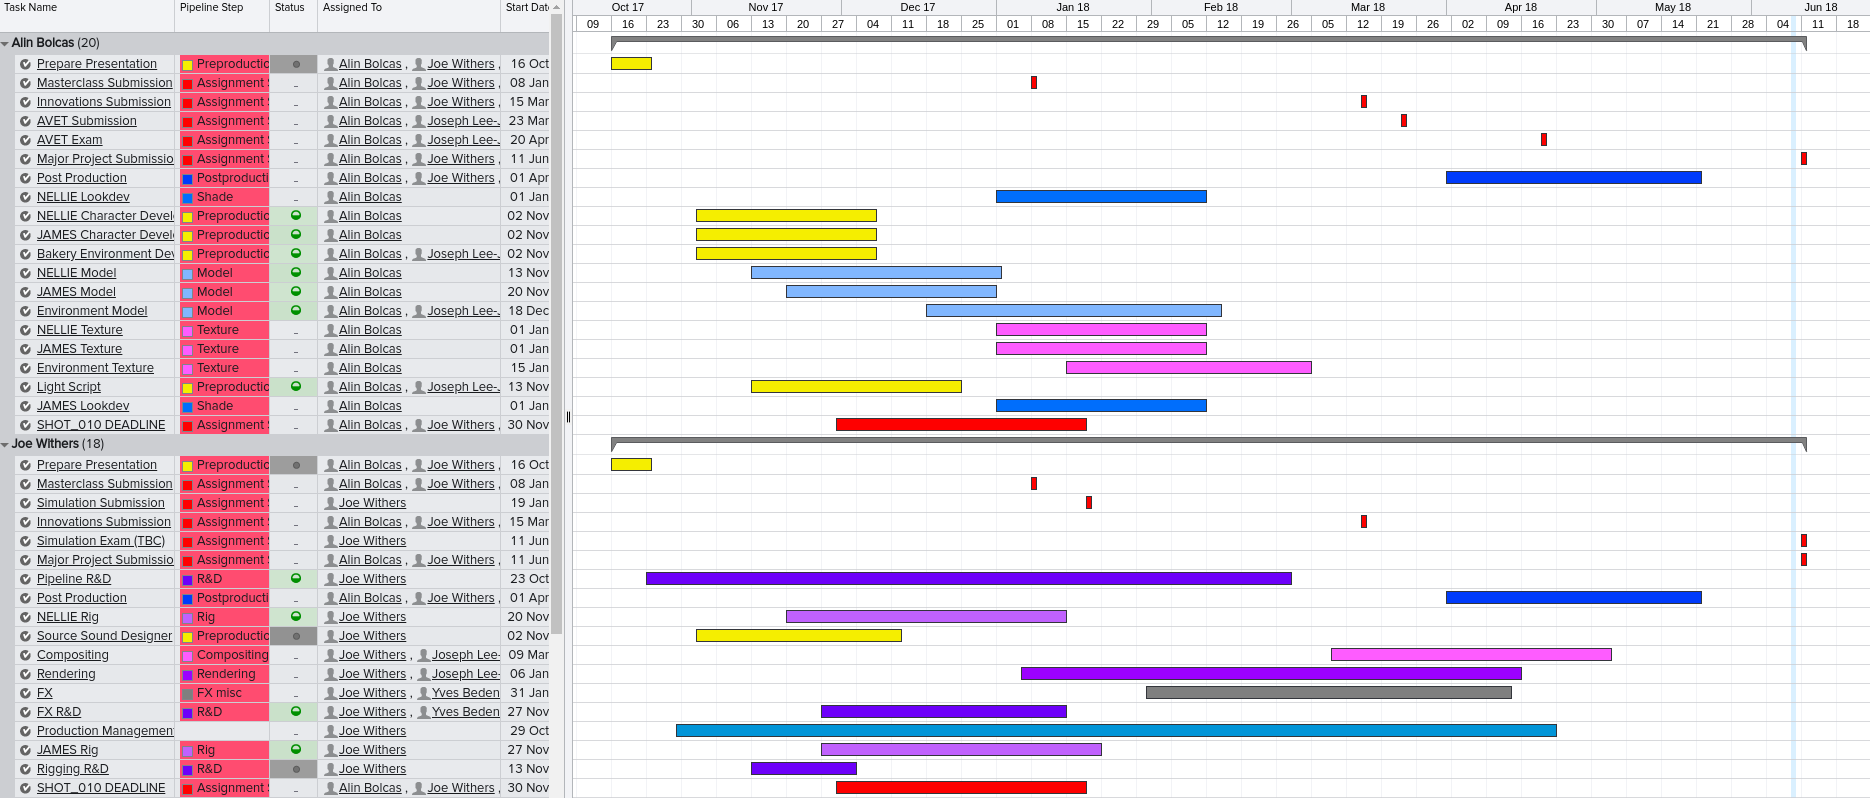
\includegraphics[width=1.0\linewidth]{images/schedule01.png}
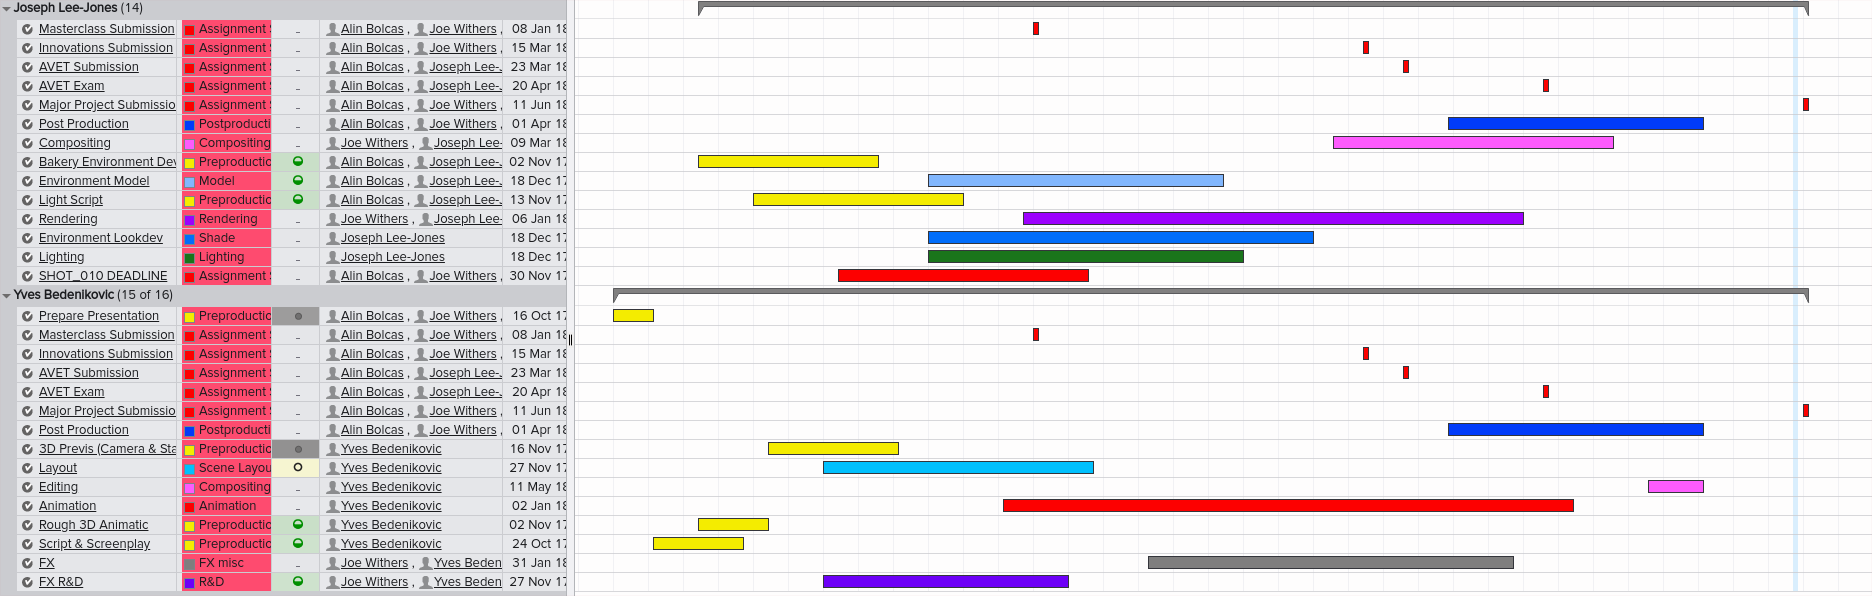
\includegraphics[width=1.0\linewidth]{images/schedule02.png}
\caption{\label{figure:schedule} The production schedule created during the first term of the project, grouped by each team member.}
\end{figure}

Unfortunately, after the first term I found it difficult to convince the other team members to continue using the Shotgun schedule, and we decided to abandon it as a result. Certain group members also found it difficult to adhere to the allocated deadlines for each task, be it a result of the scheduling of other university assignments, or a reluctance to move onto other tasks. Regrettably, this concluded my attempts at production management during the project.

\section{Character Rigging}

During this project I was responsible for the rigging of both characters, as well as the rigging of any props that the characters interact with. This proved to be quite a large demand in addition to my other responsibilities, so I sought to automate as much of this process as possible.

\subsection{Requirements}

Prior to working on the character rigs, it was important to outline features that would be required to achieve an appealing animation. This ranged from features that would allow the animator (Yves Bedenikovic) to work with them more efficiently, to features that would improve the overall aesthetic of the animation such as cloth and hair simulation. The following features were found to be of highest importance:

\begin{itemize}

\item Controls should be familiar to the animator to allow them to work intuitively with the rig. This can be achieved by using previous rigs that the animator has used as reference when setting up controllers.

\item Rigs should be capable of achieving the desired facial expressions and poses as dictated by the story.

\item Rigs should include the necessary geometry and nodes to allow for cloth simulation to be applied to clothes.

\end{itemize}

\subsection{Solution}

With these features in mind, I decided to use an automated rigging system to speed up the creation of the character rigs. This allowed me to focus primarily on the features listed above, and let a tool automate the creation of the basic bipedal rig.

I first looked at Kraken~\cite{kraken}, a rigging system included within Fabric Engine. This appealed to me as it was easily extensible through it's scripting language, which I thought I would find intuitive given that I had produced a basic automated rigging system for the specialism assignment in second year. Unfortunately, Fabric software went bankrupt at the beginning of the academic year so we were unable to get it working on the university computers.

I then found Advanced Skeleton 5~\cite{advancedSkeleton}, an extensive rigging tool for Autodesk Maya, which I found to be extremely capable and was more than adequate for my needs. This provided an additional advantage of ensuring that the control systems were consistent between both of the character rigs.

\subsection{Facial Rig}

Whilst Advanced Skeleton 5 provided a facial rig, we decided it was not suitable as the quality of the facial shapes it created were somewhat poor, and Yves Bedenikovic struggled to create appealing facial expressions using it. With this in mind we decided to take a blendshape based approach for the facial rig. By using blendshapes, a set of facial shapes could be sculpted by Alin Bolcas and art directed by Yves, which was able to more consistently give us appealing facial shapes.

I was able to combine this approach with the previous facial rig generated by Advanced Skeleton 5 for additional flexibility, however a lot of these controls were removed or hidden to reduce confusion when selecting controllers. Ultimately we found that using blendshapes caused excessive loading times for the character rigs, as there were multiple high resolution blendshape meshes needed to be loaded, though we found this to be an acceptable compromise for providing us with better facial expressions.

\section{Rendering}

For this project there were many different options for choice of renderer within Maya, however we ultimately settled on Pixar's RenderMan for multiple reasons. Initially, Solid Angle's Arnold renderer was suggested as Alin had prior experience using it, however due to licensing issues on the university machines it was ultimately not an option. Chaos Group's V-Ray was also suggested as all of the team members had previous experience using it, however it's ability to render indirect illumination is relatively poor compared to RenderMan's path tracing integrator, which was disadvantageous as our scenes relied heavily on indirect lighting due to the city street environment.

\subsection{Optimisation} \label{rlslgt}

Due to storage limits imposed by the render farm, it was necessary to cache the scene geometry to remove the need for large assets to be stored as part of the project. Whilst it would have been possible to use the Alembic file format for this, I opted to use RenderMan's RIB archive format, as it is capable of storing shading networks and render attributes in addition to scene geometry. One downside of this approach is that shaders cannot easily be changed after the cache has been made, however it eliminates the need for reassignment of shaders, which would be necessary in a comparable Alembic caching workflow.

In order to speed up this process I needed to design and develop a script that would export the entire lighting scene into RIB archives with minimal user input. In order to save storage space when caching scenes it was first important to determine which objects in the lighting scene actually required rendering, and of these objects, which were animated and thus required caching for each frame of the animation. Fortunately, Alin and Joe (Jones) had agreed on a naming convention for modelling assets, in which the names geometry objects would be suffixed with the string "\_GEO". Through the use of a single-use script, I systematically modified all of the asset build files, adding two custom attributes to every object with a name suffixed by "\_GEO". The first of these custom attributes was a boolean attribute for whether the object was to be rendered or not, and the second attribute was a boolean attribute for whether the object was animated or not. This allowed me to easily identify static and animated geometry when caching scenes, and to make changes to the contents of each cache on a per shot basis.

\begin{figure}[htbp]\centering
	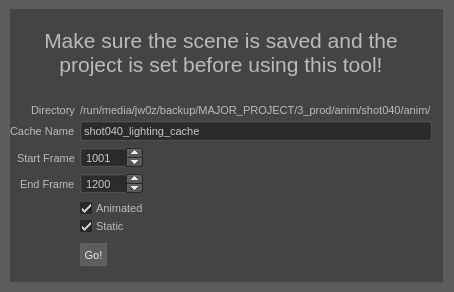
\includegraphics[width=1.0\linewidth]{images/cache_tool.png}
	\caption{\label{figure:cache_tool} The dialog used to interface with the caching script. Note that the warning was necessary to ensure caches were sent to the right location.}
\end{figure}

The lighting, camera, and XGen scalp geometry could then be exported from the lighting scene, and then be imported into a new file alongside the RIB archives to create a light weight scene file ready for rendering. To automate this process somewhat, a template 'cached' scene file was made, which included RIB archive read nodes ready to be repathed to the newly generated RIB archives. The hair shaders were also included in this file, as XGen collections would need to be applied to the scalp geometry once imported.

\subsection{Render Farming}

We intended to make use of the university render farm during this project, so testing was necessary to ensure that projects ran smoothly once submitted. I first tested a simple scene that made use of RIB archives, only to find that the version of RenderMan for Maya installed on the render farm was version 20, as opposed to version 21 which was installed in the teaching labs. This caused RIB archives to not be rendered, though was easily fixed once I had notified one of the university IT technicians.

Another issue I faced was that any absolute file paths (any file paths that are not relative to the Maya project directory), would cause errors as that path would not exist on the render farm storage server. To help solve this, I used a solution listed in a StackOverflow~\cite{stackoverflow} thread to create the script shown in Listing~\ref{lst:grep}. This script would traverse all Maya scene files in my project directory, and replace any absolute file path strings with file path strings which would work on the render farm.

Further issues relating found whilst testing XGen content on the render farm are described in section~\ref{threadsafe}.

\subsection{Distributed Rendering Tools}

Due to inconsistent availability of the render farm, our only other immediate option for rendering was to use the computers in the teaching labs. To maximise our rendering output and to minimise disruption to other students, I decided to connect to other computers remotely over SSH. This allows me to connect to far more computers than I would be physically able log into, and at the same time allows other users to log into and use the same computer.

I was able to write a short Python script which used the \texttt{ping} command to check which of the computers on the university network were online and running Linux, relying on the host name naming convention using the name of the room in which the computer is located. Upon connecting to a computer, I could then check whether another user is logged into the computer by capturing the output of the \texttt{who} command, so that I could render without impacting another user's session. In situations where a computer was found to be logged in by another user, I could check the current CPU and memory usage by capturing the output of the commands in Listing~\ref{lst:cpumem}.

As Linux does not natively support issuing commands in parallel to multiple hosts over SSH, I made use of the \texttt{parallel-ssh}\cite{pssh} Python library to provide this functionality. By following an article from \texttt{Linux.com}\cite{martin_2008}, I was able to use an array of host names combined with an array of arguments to render multiple frames using multiple hosts with ease.

Unfortunately I soon found the limit of the university network infrastructure, as having multiple computers reading from and writing to a single directory proved to extremely slow. It was therefore necessary to extend my original command to copy the project directory onto the transfer drive of that computer, execute the render, and finally copy the rendered frames back into the desired directory. Whilst this increased the time required to start a render, the speed of the render itself was much improved.

Whilst this method proved to be extremely powerful, it was certainly not reliable; If a computer is restarted into Windows it cannot be accessed over SSH, meaning that frames were often lost if someone needed to use the computer. As a result we primarily used this technique for test renders and shorter sequences, using the render farm to render shots which were known to render without error and for longer sequences.

\section{Groom}

Both of the character designs for this project required semi-realistic hair rendering, so we decided to make use of the XGen plugin within Maya. XGen was chosen as it is supported within RenderMan, and doesn't require additional licenses unlike other third party groom software such as Yeti. Unfortunately, none the team members had any experience using XGen, so we relied heavily on tutorial resources such as those published by Michael Cauchi \cite{cauchi_2017} and Jesus Fernandez \cite{fernandez_2018}. Together with Alin Bolcas, XGen collections were generated for both characters; I was responsible for setting up and configuring the XGen pipeline, with Alin being responsible for the artistic direction.

\subsection{Pipeline} \label{threadsafe}

As shown in Figure~\ref{figure:pipelineFlow}, Groom assets were not passed through the full asset pipeline, due to Maya not supporting referencing of XGen content. To solve this, the XGen collections and descriptions were exported, and later applied to Alembic caches of the scalp geometries in the cached scene for rendering.

During my initial tests for rendering XGen content using the university render farm, I found that hair would 'jump' from frame to frame and flicker uncontrollably. After a long email chain with one of the demonstrators and one of the IT technicians, we were able to determine that something in RenderMan for Maya's XGen parser was not thread safe. This resulted in incorrect memory locations being read if more than one frame was being rendered at the same time on a single machine. The solution to this was to submit render farm jobs using just one instance, but to use the same number of threads (slots) as would be allocated had we submit the job using more than a single instance. This solution had a negligible impact on render times, but had the additional benefit of reducing the likelihood of crashes, as only a single render was occupying the memory at any given time.

\section{Compositing}

In addition to being responsible for rendering, I took responsibility for compositing the shots, which was convenient as I was managing the storage of the raw renders and would be the first member of the team to get a chance to do any compositing. Being more technically inclined my compositing responsibilities mainly consisted of:

\begin{itemize}

\item Reconstructing the 'beauty' pass from the individual AOV passes. The AOVs we ended up using for reconstruction were direct diffuse, direct specular, indirect diffuse, indirect specular, subsurface, and transmissive, with the beauty pass being used for reference. The albedo pass was also used to generate a high pass filter for overall sharpening.

\item Rotopainting out any visual errors if time did not permit re-rendering a shot. This primarily consisted of hiding any intersections between the shirt and the jacket, or intersections between the cornea and the eyelid when the eyes were closed.

\item Removing Fireflies or any high variance visual noise from the individual passes, either through use of Nuke's denoiser or a third party 'Firefly Killer' gizmo found online \cite{muller_2015}.

\item Setting the view transform as ACES Filmic, and setting up a node to bake the colour space prior to writing.

\item Adding depth of field to shots where depth of field wasn't calculated in RenderMan.

\end{itemize}

\subsection{Workflow}

As these tasks were common to all shots, I created a template Nuke script which configures everything for me. Unfortunately, when reading multichannel EXRs generated by Renderman, Nuke would swap the alpha channel with the red channel from the direct specular. However this was easily fixed using a pair of copy nodes.

\begin{figure}[htbp]\centering
	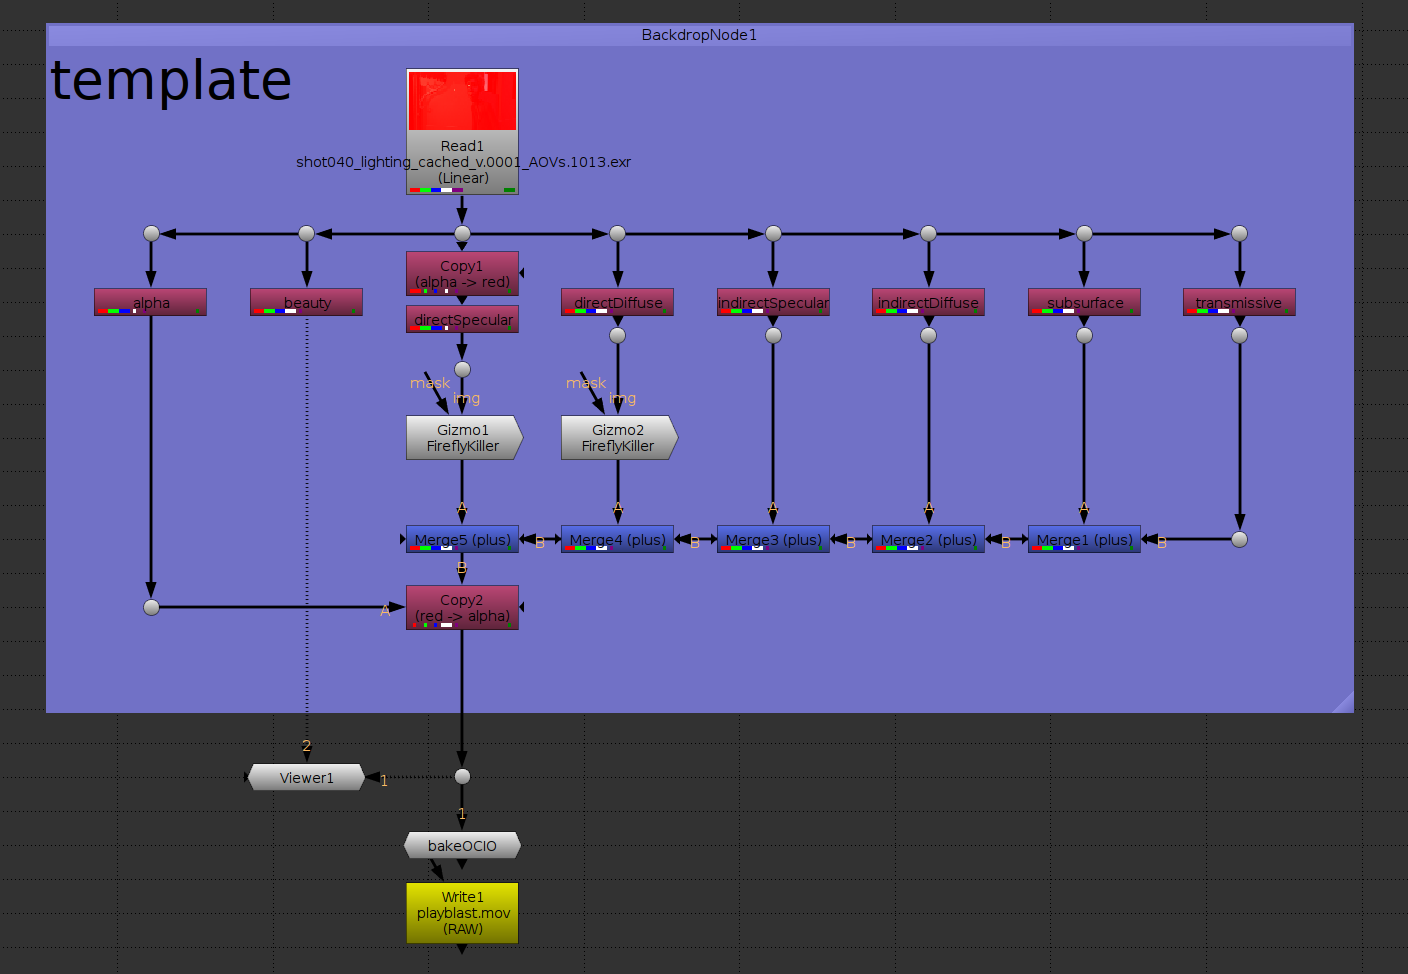
\includegraphics[width=1.0\linewidth]{images/compTemplate.png}
	\caption{\label{figure:compTemplate} The template Nuke script which was used as the basis for all shots.}
\end{figure}

As mentioned above, it was necessary to choose a view transform as RenderMan outputs images in linear colour space. The default option for this would be sRGB, however we opted to use ACES Filmic as it provides a very wide dynamic range, and avoids over-saturation of highlights on skin tones. Figure~\ref{figure:filmic} illustrates the difference between sRGB and Filmic, using one of our renders.

\begin{figure}[htbp]
\centering

\includegraphics[width=0.48\linewidth]{images/srgb_nellie.png}
\hfill

\includegraphics[width=0.48\linewidth]{images/filmic_nellie.png}
\newline
\newline

\includegraphics[width=0.48\linewidth]{images/james_srgb.png}
\hfill
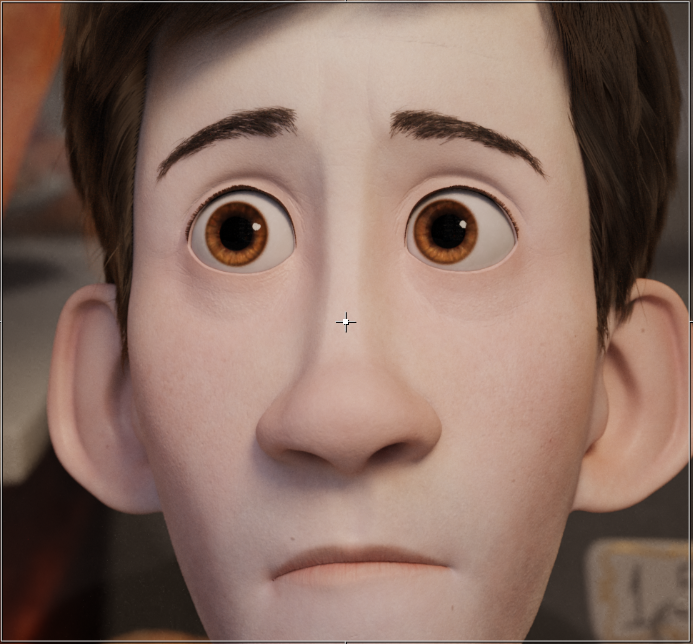
\includegraphics[width=0.48\linewidth]{images/james_filmic.png}
\caption{\label{figure:filmic} Comparison between sRGB viewing transform (Left) and Filmic 'Medium High Contrast' (Right). Note how skin highlights become over saturated in the sRGB viewing transform, giving a 'sunburned' look.}
\end{figure}

For the opening sequence (Shots 1 through 4), a more complex Nuke script was necessary as we needed to integrate FX elements, all of which were rendered separately. We also chose to render the foreground and background buildings separately so that we could make adjustments to them independently.

To integrate the snowfall FX I used alembic cached spheres generated by Yves Bedenikovic, imported directly into Nuke as shown in Figure~\ref{figure:shot010comp}. When combined with an alembic cache of the camera for the shot, I was able to make use of Nuke's scanline renderer to render the snowfall FX within Nuke, offering me greater flexibility when placing it within the scene.

\begin{figure}[htbp]\centering
	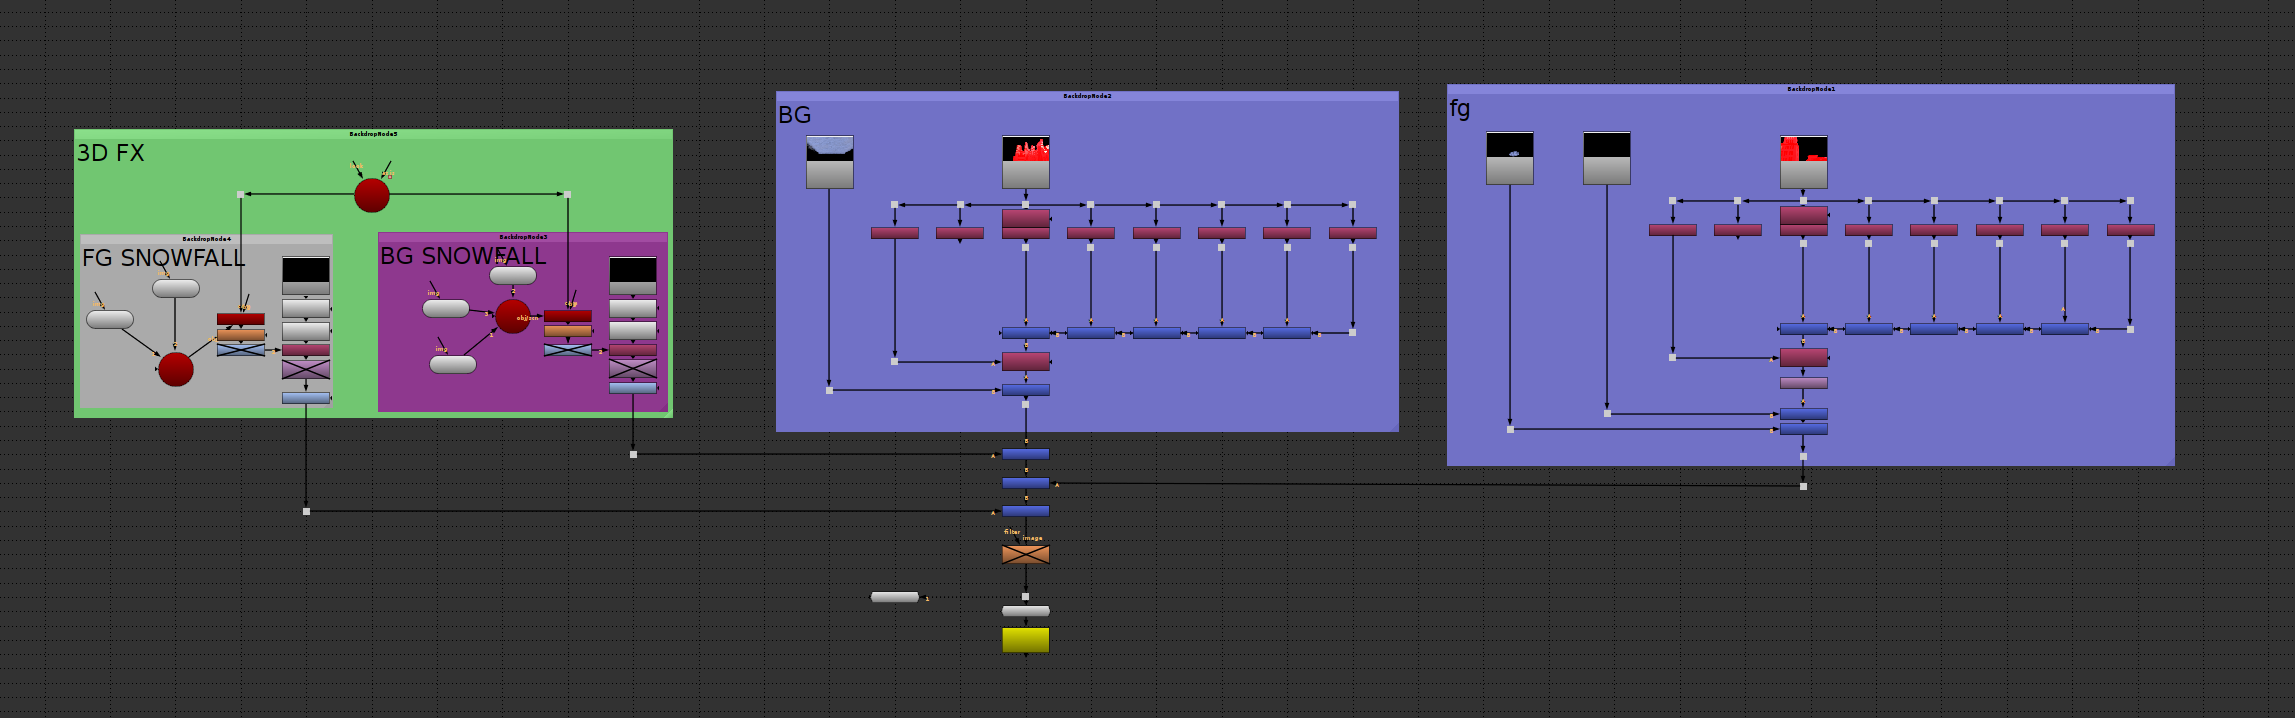
\includegraphics[width=1.0\linewidth]{images/shot010comp.png}
	\caption{\label{figure:shot010comp} The Nuke script which was used for the opening shot. Similar Nuke scripts were used for shots 2, 3, and 4 to integrate the snowfall with a great degree of flexibility.} %TODO
\end{figure}

\subsection{Results}

Figure~\ref{figure:compcomparison} shows some before and after comparisons between the 'beauty' pass from RenderMan, and the results of my compositing process. Figure~\ref{figure:shot010only} shows the output of the Nuke script described in Figure~\ref{figure:shot010comp}.

\begin{figure}[htbp]
\centering
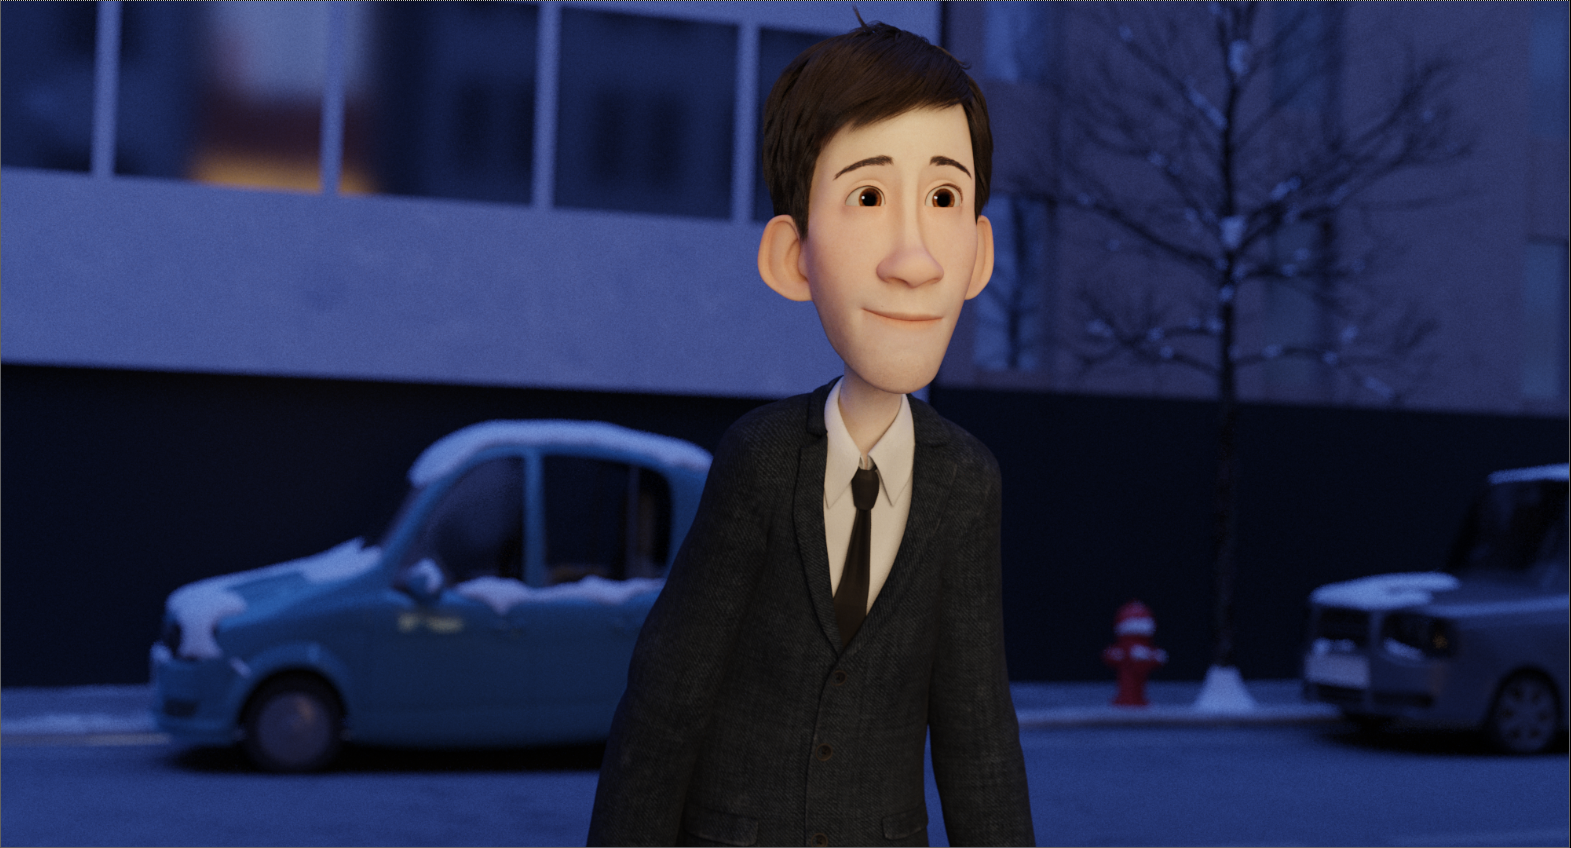
\includegraphics[width=0.48\linewidth]{images/shot020_precomp.png}
\hfill

\includegraphics[width=0.48\linewidth]{images/shot020_comp.png}
\newline
\newline

\includegraphics[width=0.48\linewidth]{images/shot030_precomp.png}
\hfill

\includegraphics[width=0.48\linewidth]{images/shot030_comp.png}
\newline
\newline

\includegraphics[width=0.48\linewidth]{images/shot040_precomp.png}
\hfill

\includegraphics[width=0.48\linewidth]{images/shot040_comp.png}
\newline
\newline

\includegraphics[width=0.48\linewidth]{images/shot070_precomp.png}
\hfill

\includegraphics[width=0.48\linewidth]{images/shot070_comp.png}
\caption{\label{figure:compcomparison} Comparison between the 'beauty' pass generated by RenderMan (Left), and the results of my compositing process (Right).}
\end{figure}

\begin{figure}[htbp]\centering
	
\includegraphics[width=1.0\linewidth]{images/shot010_comp_02.png}
	\newline
	\newline
	
\includegraphics[width=1.0\linewidth]{images/shot010_comp_01.png}
	\caption{\label{figure:shot010only} Composited frames from the opening shot.}
\end{figure}

\section{Critical Reflection}

Overall I am pleased with my major contributions to this project; I believe I have created a set of pipeline tools that improved the efficiency of this project, and could potentially be used for future student projects if required. However, at the time of writing this report the project is yet to be finished, so one has to recognise the shortcomings with the team that resulted in this situation.

As mentioned in section \ref{productionManagement}, my attempts at production management were short lived, and I feel the progression of the project was slowed as a result. I accept full responsibility for the mistakes made in this regard, but feel fortunate that it has afforded me the chance to learn from this experience. Before undertaking any future production management roles, I am now aware that I need to be far more assertive in regards to scheduling and task management. This especially applies to artists, as it seems they can easily lose sight of the 'bigger picture', as a result of being highly focused on creating work to the best of their abilities.

As far as my 'artistic' contributions are concerned, I am proud of the compositing work I was able to perform in such a short timescale, but feel my character rigging left a lot to be desired. The initial requirements for the character rig listed a cloth simulation, however although I was able to implement it into one of the rig versions, it was ultimately not used in production as it produced ugly results and would have cost a lot of time to simulate. I would have liked to have contributed more of my time to working out these issues, as I feel it would much improve the visual fidelity of the animation, especially on the aprons and James' jacket. As a result of this I had to rely on skinning the clothing, which proved to be very difficult, with intersection artefacts appearing in the final renders which required a lot of rotopainting to fix. Nonetheless, creating two human character rigs was quite a tall order even with the use of automated rigging tools, so I am somewhat satisfied that I was able to provide Yves with these in addition to my other responsibilities.

Whilst we were not able to complete all of the rendering for this project, I stand by my choice of RenderMan as renderer for this project. I instead attribute the lack of renders to the large amount of data generated by all of the assets in our scene, and the strain that it put on the university network infrastructure. Had we not have chosen a renderer with caching functionality similar to that of RenderMan's RIB archiving, I fear the scenes would take excessively long to load prior to rendering, and I sincerely doubt the project with un-cached assets would fit within the render farm's 30gb storage limit. Additionally I feel we made good use of RenderMan's path tracing integrator to produce images of a high visual standard, though I am impressed by the results I have seen achieved by other renderers such as Redshift at a significantly lower time cost.

\newpage

\bibliographystyle{plain}
\bibliography{references}

\newpage
\appendix

\begin{lstlisting}[language=bash, label={lst:cpumem}, caption={Extract from the Python script used to determine which of the computers on the university network are suitable for rendering on. By capturing the output of the following commands I was able to get the current CPU and memory usage.}]
# return the current cpu usage
top -bn1 | grep 'Cpu(s)' | sed 's/.*, *\([0-9.]*\)
# return the current memory usage
free | grep Mem | awk '{print $3/$2 * 100.0}'
\end{lstlisting}

\begin{lstlisting}[language=bash, label={lst:grep}, caption={The bash script used to replace any absolute paths in Maya scene files, and replace them with file paths suitable for use on the render farm. (Modified from this StackOverflow thread~\cite{stackoverflow})}]
grep -rl --include \*.ma "/home/i7463769/"  | xargs sed -i 's#/home/i7463769/#/render/i7463769/#g'
\end{lstlisting}

\end{document}
